\section{Capítulo 10 -- Documentação: OpenAPI, Swagger e Postman}

O TaskFlow já tem cadastro, \textit{login} e um CRUD completo de tarefas, mas só quem leu o código sabe usá-lo. Neste capítulo você vai descrever a API no formato OpenAPI, o padrão do mercado, gerando boa parte da descrição a partir dos esquemas do Zod que a própria API usa para validar; publicar uma documentação navegável com o Swagger UI, onde é possível testar cada \textit{endpoint}; e levar a API para o Postman, onde as requisições ganham variáveis, \textit{scripts} e testes automáticos, que também rodam no terminal com o Newman.

\subsection{10.1 A documentação faz parte da API}

Uma API é usada por pessoas que não estavam na sala quando ela foi projetada: quem faz o aplicativo de celular, a equipe de outra empresa, você mesmo daqui a seis meses. Para elas, a API \textbf{é} a documentação. Um \textit{endpoint} que ninguém sabe que existe, ou que ninguém sabe chamar, não serve para nada; um comportamento que não está escrito vira pergunta no suporte, ou um erro no cliente que só aparece em produção.

Uma boa documentação de API responde, para cada operação, sem que seja preciso ler o código:

\begin{itemize}
  \item qual é o método e o endereço, e o que a operação faz;
  \item como se autenticar, e quais operações dispensam a autenticação;
  \item quais parâmetros e qual corpo ela aceita, com os tipos, os campos obrigatórios e os limites, como ``título de até 120 caracteres'';
  \item o que ela devolve no sucesso, com o código de status e o formato do corpo;
  \item quais erros podem acontecer, com o status e o formato de cada um, e não só o caminho feliz;
  \item as regras gerais, como o formato das datas, a paginação e decisões como ``dados inválidos recebem sempre \texttt{400}'', que o Capítulo 8 pediu para registrar.
\end{itemize}

Escrever tudo isso à mão, em um documento de texto, tem dois problemas: cada ferramenta precisaria de alguém para lê-lo, e ele se desatualiza na primeira mudança do código. A solução do mercado é descrever a API em um formato que \textbf{programas} entendem.

\subsection{10.2 OpenAPI e Swagger}

A \textbf{Especificação OpenAPI} define um formato, em JSON ou YAML, para descrever APIs HTTP: os endereços, os métodos, os parâmetros, os corpos, as respostas e a autenticação. Ela nasceu em 2011 com o nome de Swagger, criada para documentar a API de um dicionário \textit{online}. Em 2015, a especificação foi doada à OpenAPI Initiative, mantida pela Linux Foundation, e passou a se chamar OpenAPI; a versão 3.0 saiu em 2017, a 3.1, que alinhou os esquemas ao padrão JSON Schema, em 2021, e a 3.2 em 2025. O nome Swagger ficou com as ferramentas criadas em torno do formato, como o \textbf{Swagger UI}, que transforma um documento OpenAPI em uma página navegável, e o Swagger Editor.

Com um documento OpenAPI, uma única descrição alimenta várias ferramentas: páginas de documentação, como o Swagger UI, o Redoc e o Scalar; clientes de teste, como o Postman e o Insomnia, que importam todas as requisições de uma vez; geradores de código, que criam o cliente da API em TypeScript, Java, Kotlin ou Swift; validadores, que conferem se a API responde o que promete; e até assistentes de IA, que leem o documento para descobrir como chamar a API. É o ``contrato'' do Capítulo 1, que no SOAP era o WSDL, obrigatório, e no REST é opcional, mas é praticamente um padrão de fato.

Há duas formas de trabalhar com o documento:

\begin{itemize}
  \item \textbf{\textit{Design-first}} (primeiro o desenho): o documento é escrito antes do código, discutido entre as equipes, e o código é feito para cumpri-lo. Combina com APIs públicas e com equipes que trabalham em paralelo, como o Capítulo 2 sugeriu.
  \item \textbf{\textit{Code-first}} (primeiro o código): o documento é gerado, no todo ou em parte, a partir do código. Combina com projetos em que a mesma equipe faz a API e a mantém, e tem uma grande vantagem: o que vem do código não se desatualiza.
\end{itemize}

O TaskFlow já existe, então vai pelo segundo caminho, aproveitando os esquemas do Zod, que já descrevem exatamente o que a API aceita.

\subsection{10.3 A estrutura de um documento OpenAPI}

Antes de gerar o documento, vale ver como ele é. Este é um trecho, em YAML, que descreve uma única operação, a busca de uma tarefa:

\begin{codigo}
\begin{Verbatim}[breaklines=true, breaksymbolleft={}, fontsize=\footnotesize]
openapi: 3.1.0
info:
  title: TaskFlow API
  version: 1.0.0
paths:
  /api/tasks/{id}:
    get:
      summary: Busca uma tarefa
      parameters:
        - name: id
          in: path
          required: true
          schema:
            type: string
      responses:
        "200":
          description: A tarefa
          content:
            application/json:
              schema:
                $ref: "#/components/schemas/Tarefa"
        "404":
          description: A tarefa não existe ou não é sua
components:
  schemas:
    Tarefa:
      type: object
      properties:
        id: { type: string }
        title: { type: string }
\end{Verbatim}
\end{codigo}

O YAML representa os mesmos dados que um JSON, usando a indentação no lugar das chaves; a lista de parâmetros, com o \texttt{-}, é um vetor. As partes principais de um documento são estas:

\begin{center}
\begin{tabular}{@{}P{0.24\linewidth}P{0.66\linewidth}@{}}
\toprule
\rowcolor{headergray}
\tblheader{Campo} & \tblheader{Conteúdo} \\
\midrule
\texttt{openapi} & a versão da especificação usada no documento \\
\rowcolor{rowgray} \texttt{info} & o nome, a versão da API e uma descrição geral \\
\texttt{servers} & os endereços onde a API está no ar \\
\rowcolor{rowgray} \texttt{paths} & cada endereço, com as operações (\texttt{get}, \texttt{post}...) e, em cada uma, os \texttt{parameters}, o \texttt{requestBody} e as \texttt{responses} \\
\texttt{components} & as partes reaproveitáveis: \texttt{schemas}, \texttt{responses}, \texttt{securitySchemes} \\
\rowcolor{rowgray} \texttt{security} & a autenticação exigida, para todas as operações ou para cada uma \\
\texttt{tags} & grupos de operações, usados para organizar a página \\
\bottomrule
\end{tabular}
\end{center}

O \texttt{\$ref} é uma referência: em vez de repetir a descrição da tarefa em todas as respostas que a devolvem, cada uma aponta para \texttt{\#/components/schemas/Tarefa}, e a descrição fica em um lugar só. Os esquemas, dentro de \texttt{schema}, seguem o \textbf{JSON Schema}, um padrão para descrever o formato de dados JSON, com \texttt{type}, \texttt{properties}, \texttt{required}, \texttt{minLength}, \texttt{enum} e outras palavras-chave. Os códigos de status ficam entre aspas porque, em YAML e JSON, as chaves de um objeto são textos.

\subsection{10.4 Do Zod para o JSON Schema}

O Zod 4 converte um esquema em JSON Schema com a função \texttt{z.toJSONSchema}. Este é o resultado para o \texttt{esquemaNovaTarefa} do Capítulo 6, com a expressão regular da data abreviada:

\begin{codigo}
\begin{Verbatim}[breaklines=true, breaksymbolleft={}, fontsize=\footnotesize]
z.toJSONSchema(esquemaNovaTarefa, { io: "input" });
// {
//   "type": "object",
//   "properties": {
//     "title": { "type": "string",
//                "minLength": 1, "maxLength": 120 },
//     "description": { "anyOf": [
//       { "type": "string", "maxLength": 2000 },
//       { "type": "null" } ] },
//     "status": { "type": "string",
//                 "enum": ["PENDING", "IN_PROGRESS", "DONE"] },
//     "priority": { "type": "string",
//                   "enum": ["LOW", "MEDIUM", "HIGH"] },
//     "dueDate": { "anyOf": [
//       { "type": "string", "format": "date",
//         "pattern": "^(?:(?:\\d\\d[2468][048]|..." },
//       { "type": "null" } ] }
//   },
//   "required": ["title"]
// }
\end{Verbatim}
\end{codigo}

Os limites, os valores aceitos pelos \texttt{enum}, o campo obrigatório e o \texttt{nullable}, que virou ``texto ou \texttt{null}'', estão todos lá, sem nenhuma linha escrita à mão. A opção \texttt{io: "input"} pede a descrição da \textbf{entrada}, o que o cliente envia, e não da saída. A diferença aparece na data: o cliente envia o texto \texttt{"2026-12-01"}, e o \texttt{transform} só o converte em \texttt{Date} depois da validação. Sem essa opção, o Zod se recusa a converter esquemas com \texttt{transform}, porque um \texttt{Date} não tem representação em JSON.

A conversão tem limites, e eles valem para qualquer gerador. Uma regra escrita como função, no \texttt{refine}, não pode ser traduzida, e por isso o limite de 72 bytes da senha (Capítulo 9) não aparece. No \texttt{pipe}, a descrição da entrada mostra só o primeiro esquema, e por isso o e-mail do cadastro aparece como um texto qualquer, sem o formato de e-mail. O que o gerador não alcança vai para o texto da descrição, como você verá a seguir.

\subsection{10.5 O documento do TaskFlow}

Todo o documento fica em um arquivo, \texttt{lib/openapi.ts}. A primeira parte importa os esquemas e define uma função que os converte:

\begin{codigo}
\begin{Verbatim}[breaklines=true, breaksymbolleft={}, fontsize=\footnotesize]
// lib/openapi.ts -- a documentação da API, no formato OpenAPI 3.1
import * as z from "zod";
import {
  Priority,
  TaskStatus,
} from "@/app/generated/prisma/client";
import {
  esquemaEdicaoTarefa,
  esquemaFiltros,
  esquemaNovaTarefa,
} from "@/lib/esquemas/tarefas";
import {
  esquemaCadastro,
  esquemaLogin,
} from "@/lib/esquemas/auth";

// Converte um esquema do Zod em JSON Schema. O io: "input"
// descreve o que o cliente envia, antes dos transform.
function jsonSchema(esquema: z.ZodType) {
  const resultado = z.toJSONSchema(esquema, { io: "input" });
  delete resultado.$schema;
  return resultado;
}
\end{Verbatim}
\end{codigo}

O \texttt{delete} remove o campo \texttt{\$schema}, que o \texttt{toJSONSchema} acrescenta para dizer qual versão do JSON Schema foi usada; dentro de um documento OpenAPI, ele é desnecessário. As respostas da API, ao contrário das entradas, não têm esquemas do Zod: elas são montadas pelo Prisma, com o \texttt{select} do Capítulo 5. Para documentá-las, o mais simples é descrevê-las com o próprio Zod, só para gerar o JSON Schema:

\begin{codigo}
\begin{Verbatim}[breaklines=true, breaksymbolleft={}, fontsize=\footnotesize]
// O que a API devolve (não há esquema do Zod para isso: as
// respostas são montadas pelo Prisma, com o select)
const tarefa = z.object({
  id: z.string(),
  title: z.string(),
  description: z.string().nullable(),
  status: z.enum(TaskStatus),
  priority: z.enum(Priority),
  dueDate: z.iso.datetime().nullable(),
  createdAt: z.iso.datetime(),
  updatedAt: z.iso.datetime(),
});

const listaDeTarefas = z.object({
  data: z.array(tarefa),
  meta: z.object({
    page: z.int(),
    limit: z.int(),
    total: z.int(),
    totalPages: z.int(),
  }),
});

const usuario = z.object({
  id: z.string(),
  name: z.string(),
  email: z.email(),
  createdAt: z.iso.datetime(),
});

const token = z.object({
  token: z.string(),
  tokenType: z.literal("Bearer"),
  expiresIn: z.int(),
});

const problema = z.object({
  title: z.string(),
  status: z.int(),
  detail: z.string(),
  errors: z.record(z.string(), z.array(z.string())).optional(),
  instance: z.string().optional(),
});
\end{Verbatim}
\end{codigo}

O \texttt{z.int()} descreve um número inteiro; o \texttt{z.iso.datetime()}, uma data e hora no formato ISO 8601, como as que o JSON da API traz; o \texttt{z.literal("Bearer")}, um campo que só pode ter aquele valor; e o \texttt{z.record}, um objeto com chaves quaisquer, como o \texttt{errors} do Capítulo 8, em que cada campo tem uma lista de mensagens. Estes esquemas nunca validam nada, só descrevem: se o \texttt{camposTarefa} ganhar um campo, este esquema precisa ser atualizado à mão, um ponto de atenção que volta na Seção 10.10.

Como as mesmas estruturas aparecem em muitas operações, algumas funções curtas evitam a repetição:

\begin{codigo}
\begin{Verbatim}[breaklines=true, breaksymbolleft={}, fontsize=\footnotesize]
// Atalhos para não repetir as mesmas estruturas
const ref = (nome: string) => ({
  $ref: `#/components/schemas/${nome}`,
});
const emJson = (nome: string) => ({
  content: { "application/json": { schema: ref(nome) } },
});
const erro = (descricao: string) => ({
  description: descricao,
  content: {
    "application/problem+json": { schema: ref("Problema") },
  },
});
const comum = (nome: string) => ({
  $ref: `#/components/responses/${nome}`,
});

// Os filtros da listagem viram parâmetros da query string
const filtros = jsonSchema(esquemaFiltros);
const parametrosDaLista = Object.entries(
  filtros.properties ?? {},
).map(([name, schema]) => ({ name, in: "query", schema }));
\end{Verbatim}
\end{codigo}

A \texttt{ref} monta uma referência a um esquema; a \texttt{emJson} diz que o corpo é JSON e segue esse esquema; a \texttt{erro} descreve uma resposta de erro no formato \texttt{application/problem+json}; e a \texttt{comum} aponta para uma das respostas reaproveitáveis, definidas no fim do documento. No OpenAPI, os parâmetros da \textit{query string} não são um objeto, como no Zod, mas uma lista, com um item por parâmetro. O \texttt{Object.entries} transforma cada propriedade do esquema dos filtros, do Capítulo 7, em um parâmetro \texttt{in: "query"}. Agora, o documento, começando pelas informações gerais e pela autenticação:

\begin{codigo}
\begin{Verbatim}[breaklines=true, breaksymbolleft={}, fontsize=\footnotesize]
export const documento = {
  openapi: "3.1.0",
  info: {
    title: "TaskFlow API",
    version: "1.0.0",
    description:
      "API de tarefas. Faça login em POST /api/auth/login e "
      + "envie o token no cabeçalho Authorization: Bearer. "
      + "Os erros seguem a RFC 9457 (Problem Details); dados "
      + "inválidos recebem sempre 400, nunca 422.",
  },
  servers: [
    {
      url: "http://localhost:3000",
      description: "Desenvolvimento",
    },
  ],
  tags: [
    { name: "Autenticação", description: "Cadastro e login" },
    { name: "Tarefas", description: "As tarefas de quem pede" },
  ],
  // Vale para todas as operações, menos as que dizem o contrário
  security: [{ bearer: [] }],
  paths: {
    "/api/auth/register": {
      post: {
        tags: ["Autenticação"],
        operationId: "cadastrar",
        summary: "Cria uma conta",
        description: "A senha precisa ter de 8 a 72 bytes.",
        security: [],
        requestBody: { required: true, ...emJson("Cadastro") },
        responses: {
          "201": {
            description: "Conta criada",
            ...emJson("Usuario"),
          },
          "400": comum("Invalido"),
          "409": erro("O e-mail já está em uso"),
        },
      },
    },
    "/api/auth/login": {
      post: {
        tags: ["Autenticação"],
        operationId: "entrar",
        summary: "Troca e-mail e senha por um token",
        description: "O token vale por 1 hora (expiresIn).",
        security: [],
        requestBody: { required: true, ...emJson("Login") },
        responses: {
          "200": {
            description: "Login feito",
            ...emJson("Token"),
          },
          "400": comum("Invalido"),
          "401": erro("E-mail ou senha incorretos"),
        },
      },
    },
\end{Verbatim}
\end{codigo}

O \texttt{security} do nível de cima vale para todas as operações: todas exigem o esquema \texttt{bearer}, definido no fim do documento. O cadastro e o \textit{login} dizem o contrário com \texttt{security: []}, uma lista vazia, ``nenhuma autenticação''. O \texttt{operationId} é um nome único para cada operação, usado pelos geradores de código, que criam funções como \texttt{cadastrar()} e \texttt{entrar()}. A descrição do cadastro completa o que a conversão não alcançou, o limite de bytes da senha, e a descrição geral, em \texttt{info}, registra a regra do \texttt{400}, como o Capítulo 8 pediu. As tarefas:

\begin{codigo}
\begin{Verbatim}[breaklines=true, breaksymbolleft={}, fontsize=\footnotesize]
    "/api/tasks": {
      get: {
        tags: ["Tarefas"],
        operationId: "listarTarefas",
        summary: "Lista as tarefas, com filtros e paginação",
        parameters: parametrosDaLista,
        responses: {
          "200": {
            description: "Uma página de tarefas",
            ...emJson("ListaDeTarefas"),
          },
          "400": comum("Invalido"),
          "401": comum("NaoAutenticado"),
        },
      },
      post: {
        tags: ["Tarefas"],
        operationId: "criarTarefa",
        summary: "Cria uma tarefa",
        requestBody: { required: true, ...emJson("NovaTarefa") },
        responses: {
          "201": {
            description: "Tarefa criada",
            headers: {
              Location: {
                description: "O endereço da tarefa criada",
                schema: { type: "string" },
              },
            },
            ...emJson("Tarefa"),
          },
          "400": comum("Invalido"),
          "401": comum("NaoAutenticado"),
        },
      },
    },
    "/api/tasks/{id}": {
      parameters: [
        {
          name: "id",
          in: "path",
          required: true,
          schema: { type: "string" },
        },
      ],
      get: {
        tags: ["Tarefas"],
        operationId: "buscarTarefa",
        summary: "Busca uma tarefa",
        responses: {
          "200": { description: "A tarefa", ...emJson("Tarefa") },
          "401": comum("NaoAutenticado"),
          "404": comum("NaoEncontrada"),
        },
      },
      patch: {
        tags: ["Tarefas"],
        operationId: "editarTarefa",
        summary: "Altera os campos enviados",
        requestBody: {
          required: true,
          ...emJson("EdicaoTarefa"),
        },
        responses: {
          "200": {
            description: "A tarefa atualizada",
            ...emJson("Tarefa"),
          },
          "400": comum("Invalido"),
          "401": comum("NaoAutenticado"),
          "404": comum("NaoEncontrada"),
        },
      },
      delete: {
        tags: ["Tarefas"],
        operationId: "excluirTarefa",
        summary: "Exclui uma tarefa",
        responses: {
          "204": { description: "Excluída (sem corpo)" },
          "401": comum("NaoAutenticado"),
          "404": comum("NaoEncontrada"),
        },
      },
    },
  },
\end{Verbatim}
\end{codigo}

O caminho \texttt{/api/tasks/\{id\}} usa chaves para a parte variável, onde o Next.js usa colchetes, e declara o parâmetro \texttt{id} uma única vez, para as três operações. A criação documenta também o cabeçalho \texttt{Location} da resposta. Cada operação lista só os erros que pode dar: a busca não tem corpo, então não responde \texttt{400}. Por fim, os componentes:

\begin{codigo}
\begin{Verbatim}[breaklines=true, breaksymbolleft={}, fontsize=\footnotesize]
  components: {
    securitySchemes: {
      bearer: {
        type: "http",
        scheme: "bearer",
        bearerFormat: "JWT",
      },
    },
    schemas: {
      Cadastro: jsonSchema(esquemaCadastro),
      Login: jsonSchema(esquemaLogin),
      NovaTarefa: jsonSchema(esquemaNovaTarefa),
      EdicaoTarefa: jsonSchema(esquemaEdicaoTarefa),
      Tarefa: jsonSchema(tarefa),
      ListaDeTarefas: jsonSchema(listaDeTarefas),
      Usuario: jsonSchema(usuario),
      Token: jsonSchema(token),
      Problema: jsonSchema(problema),
    },
    responses: {
      Invalido: erro("Dados inválidos; veja o campo errors"),
      NaoAutenticado: erro("Token ausente, inválido ou vencido"),
      NaoEncontrada: erro("A tarefa não existe ou não é sua"),
    },
  },
};
\end{Verbatim}
\end{codigo}

O \texttt{securitySchemes} diz que a autenticação é HTTP do tipo \texttt{bearer}, com um JWT; é isso que faz as ferramentas mostrarem um campo para colar o \textit{token}. Os esquemas de entrada vêm do Zod, os de saída, dos esquemas descritivos acima. As três respostas comuns são as que mais se repetem: o \texttt{400}, o \texttt{401} e o \texttt{404}.

\subsection{10.6 Publicando o documento e o Swagger UI}

O documento é servido por uma rota, no endereço que as ferramentas costumam procurar:

\begin{codigo}
\begin{Verbatim}[breaklines=true, breaksymbolleft={}, fontsize=\footnotesize]
// app/api/openapi.json/route.ts -- o documento OpenAPI da API
import { documento } from "@/lib/openapi";

export function GET() {
  return Response.json(documento);
}
\end{Verbatim}
\end{codigo}

O nome da pasta, \texttt{openapi.json}, vira o endereço \texttt{/api/openapi.json}. A rota não usa a requisição, então o Next.js a gera uma vez, no \textit{build}, e serve o resultado pronto. Para as pessoas, a documentação navegável fica em \texttt{/docs}, fora de \texttt{/api}, porque é uma página, e não parte da API:

\begin{codigo}
\begin{Verbatim}[breaklines=true, breaksymbolleft={}, fontsize=\footnotesize]
// app/docs/route.ts -- a documentação navegável (Swagger UI)
const cdn = "https://cdn.jsdelivr.net/npm/swagger-ui-dist@5.33.1";

const pagina = `<!doctype html>
<html lang="pt-BR">
<head>
  <meta charset="utf-8">
  <title>TaskFlow API</title>
  <link rel="stylesheet" href="${cdn}/swagger-ui.css">
</head>
<body>
  <div id="swagger-ui"></div>
  <script src="${cdn}/swagger-ui-bundle.js"></script>
  <script>
    SwaggerUIBundle({
      url: "/api/openapi.json",
      dom_id: "#swagger-ui",
      persistAuthorization: true,
    });
  </script>
</body>
</html>`;

export function GET() {
  return new Response(pagina, {
    headers: { "Content-Type": "text/html; charset=utf-8" },
  });
}
\end{Verbatim}
\end{codigo}

A rota devolve uma página HTML que carrega o Swagger UI de uma CDN, o jsDelivr, com a versão fixada no endereço, e manda o Swagger UI ler o \texttt{/api/openapi.json}. A opção \texttt{persistAuthorization} guarda o \textit{token} no navegador, para que ele não se perca ao recarregar a página. Com o servidor no ar, abra \texttt{http://localhost:3000/docs}:

\begin{center}
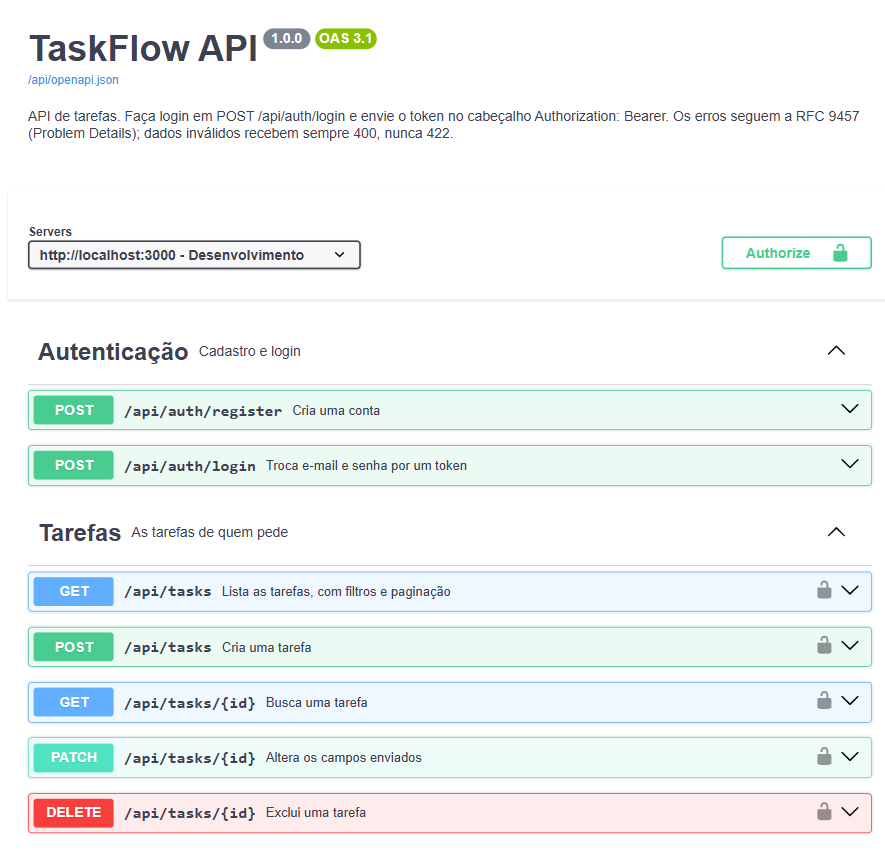
\includegraphics[width=0.95\linewidth,keepaspectratio]{imagens/capitulo-10_swagger.png}
\end{center}

As operações aparecem agrupadas pelas \texttt{tags}, e as que exigem autenticação têm um cadeado. Clicando em uma operação, aparecem os parâmetros, o corpo, com um exemplo montado a partir do esquema, e as respostas possíveis, com os seus formatos. Para usar a API pela página, este roteiro foi seguido com o TaskFlow:

\begin{enumerate}
  \item Em \texttt{POST /api/auth/login}, clique em \textbf{Try it out}, troque o exemplo do corpo por \texttt{\{"email": "demo@taskflow.com", "password": "senha123"\}} e clique em \textbf{Execute}. A resposta, \texttt{200}, traz o \textit{token}.
  \item Copie o \textit{token}, sem as aspas, clique em \textbf{Authorize}, no alto da página, cole-o no campo \texttt{Value} e confirme. Os cadeados se fecham.
  \item Em \texttt{GET /api/tasks}, clique em \textbf{Try it out}, preencha \texttt{limit} com \texttt{2} e clique em \textbf{Execute}. A resposta foi \texttt{200}, com as duas primeiras tarefas da demo.
\end{enumerate}

Abaixo de cada resposta, o Swagger UI mostra o comando \texttt{curl} equivalente, já com o cabeçalho \texttt{Authorization: Bearer ...}, útil para repetir a chamada no terminal. Repare que ele enviou também \texttt{sort=-createdAt\&page=1}: são os valores padrão do esquema dos filtros, que a página preenche sozinha.

Também vale conferir se o documento segue a especificação. O Redocly CLI, um validador de linha de comando, lê o documento e aponta os problemas:

\begin{codigo}
\begin{Verbatim}[breaklines=true, breaksymbolleft={}, fontsize=\footnotesize]
$ npx @redocly/cli lint http://localhost:3000/api/openapi.json
warning  info-license           Info object should contain
                                `license` field.
warning  no-server-example.com  Server `url` should not point
                                to example.com or localhost.
Woohoo! Your API description is valid.
\end{Verbatim}
\end{codigo}

O documento é válido. Os dois avisos são recomendações de estilo: uma licença, que faz sentido em APIs públicas, e um servidor de produção, que o TaskFlow ganha no Capítulo 12. Sem o \texttt{servers}, o validador acusaria um erro, e sem os \texttt{operationId}, sete avisos, um por operação; é por isso que eles estão no documento.

\begin{destaque}{Atenção: a documentação em produção}
A rota \texttt{/docs} mostra a todos os endereços e formatos da API. Para uma API pública, isso é desejável. Para uma API interna, avalie se a documentação deve ficar só no ambiente de desenvolvimento, ou atrás de um \textit{login}. Esconder a documentação, porém, não protege nada: a segurança vem da autenticação e da autorização, e um atacante descobre os endereços observando o tráfego do próprio aplicativo. A página também carrega código de um servidor externo, a CDN; o Capítulo 12 mostra como limitar de onde uma página pode carregar código.
\end{destaque}

\subsection{10.7 A API no Postman}

O \textbf{Postman} é o programa gráfico mais usado para trabalhar com APIs: monta requisições, guarda-as em coleções, gerencia variáveis e roda testes. Ele tem versão para Windows, macOS e Linux e uma versão \textit{web}, que precisa de um pequeno agente instalado para chamar endereços como \texttt{localhost}. Em vez de criar as requisições uma a uma, importe o documento OpenAPI:

\begin{enumerate}
  \item Com o servidor no ar, clique em \textbf{Import}, cole o endereço do documento, \texttt{/api/openapi.json} depois de \texttt{http://localhost:3000}, e confirme. O Postman lê o documento e cria uma \textbf{coleção} chamada \texttt{TaskFlow API}, com uma pasta para cada \textit{tag} e uma requisição para cada operação, nomeada pelo \texttt{summary}.
  \item Abra a coleção, na aba \textbf{Variables}: lá está a variável \texttt{baseUrl}, com o valor \texttt{http://localhost:3000}, tirado do \texttt{servers}. Todas as requisições usam \texttt{\{\{baseUrl\}\}/api/...}; para chamar outro servidor, basta mudar a variável.
  \item Na aba \textbf{Authorization} da coleção, o tipo já é \textbf{Bearer Token}, com o valor \texttt{\{\{bearerToken\}\}}, tirado do \texttt{securitySchemes}. As requisições, com \textbf{Inherit auth from parent}, herdam essa configuração.
\end{enumerate}

As chaves duplas, \texttt{\{\{nome\}\}}, marcam uma variável, substituída pelo valor no momento do envio. Além das variáveis da coleção, o Postman tem \textbf{ambientes} (\textit{environments}), conjuntos de variáveis que se trocam de uma vez, como ``TaskFlow local'' e ``TaskFlow produção'', cada um com o seu \texttt{baseUrl}; quando a mesma variável existe nos dois lugares, vale a do ambiente selecionado.

A importação monta tudo a partir dos esquemas, então algumas coisas precisam de ajuste, como aconteceu nos testes com o TaskFlow:

\begin{itemize}
  \item os corpos vêm com marcadores, como \texttt{\{"email": "<string>", "password": "<string>"\}}, que precisam ser trocados por dados de verdade;
  \item na listagem, todos os parâmetros da \textit{query string} vêm marcados, com valores de exemplo: \texttt{status=PENDING}, \texttt{search=<string>}. Desmarque os que não for usar; esquecido, o \texttt{search} procura tarefas com o texto \texttt{<string>} no título, e a lista vem vazia;
  \item o \texttt{:id} das requisições de uma tarefa vem vazio, na aba \textbf{Params}.
\end{itemize}

\subsection{10.8 Scripts e testes no Postman}

Copiar o \textit{token} do \textit{login} para a coleção, à mão, a cada hora, cansa. No Postman, cada requisição tem uma aba \textbf{Scripts}, com duas partes: \textbf{Pre-request}, que roda antes do envio, e \textbf{Post-response}, que roda depois que a resposta chega. Os \textit{scripts} são escritos em JavaScript, com o objeto \texttt{pm}, que dá acesso à resposta e às variáveis. No \textit{login}, com o corpo \texttt{\{"email": "demo@taskflow.com", "password": "senha123"\}}, o \textit{script} de Post-response é este:

\begin{codigo}
\begin{Verbatim}[breaklines=true, breaksymbolleft={}, fontsize=\footnotesize]
pm.test("login responde 200 com o token", () => {
  pm.response.to.have.status(200);
  pm.expect(pm.response.json().token).to.be.a("string");
});
// guarda o token: a coleção usa {{bearerToken}} no Bearer
const { token } = pm.response.json();
pm.collectionVariables.set("bearerToken", token);
\end{Verbatim}
\end{codigo}

O \texttt{pm.test} registra um teste, com um nome e uma função; se a função lançar um erro, o teste falha. Dentro dela, as conferências usam o estilo da biblioteca Chai, que se lê quase como uma frase: ``a resposta deve ter o status 200'', ``o \textit{token} deve ser um texto''. As duas últimas linhas guardam o \textit{token} na variável que a coleção usa no Bearer. A partir daí, basta fazer o \textit{login} uma vez, e todas as requisições de tarefas saem autenticadas.

A mesma ideia encadeia as requisições de uma tarefa. Na criação, com o corpo \texttt{\{"title": "Testar no Postman", "priority": "HIGH"\}}, o \textit{script} guarda o \texttt{id} da tarefa criada:

\begin{codigo}
\begin{Verbatim}[breaklines=true, breaksymbolleft={}, fontsize=\footnotesize]
pm.test("cria com 201 e Location", () => {
  pm.response.to.have.status(201);
  pm.response.to.have.header("Location");
});
// guarda o id para as próximas requisições
pm.collectionVariables.set("tarefaId", pm.response.json().id);
\end{Verbatim}
\end{codigo}

Nas requisições de busca, edição e exclusão, o valor do \texttt{:id}, na aba Params, passa a ser \texttt{\{\{tarefaId\}\}}. Os \textit{scripts} delas conferem o resultado:

\begin{codigo}
\begin{Verbatim}[breaklines=true, breaksymbolleft={}, fontsize=\footnotesize]
pm.test("busca a tarefa criada", () => {
  pm.response.to.have.status(200);
  pm.expect(pm.response.json().title).to.eql("Testar no Postman");
});
\end{Verbatim}
\end{codigo}

\begin{codigo}
\begin{Verbatim}[breaklines=true, breaksymbolleft={}, fontsize=\footnotesize]
pm.test("marca a tarefa como DONE", () => {
  pm.response.to.have.status(200);
  pm.expect(pm.response.json().status).to.eql("DONE");
});
\end{Verbatim}
\end{codigo}

O \textit{script} da edição supõe o corpo \texttt{\{"status": "DONE"\}}, e a exclusão confere o \texttt{204}. Os testes de erro são tão importantes quanto os de sucesso. Uma cópia da listagem, com a autorização trocada para \textbf{No Auth}, confere se a API recusa quem não tem \textit{token}, e no formato certo:

\begin{codigo}
\begin{Verbatim}[breaklines=true, breaksymbolleft={}, fontsize=\footnotesize]
pm.test("sem token: 401 no formato Problem Details", () => {
  pm.response.to.have.status(401);
  pm.response.to.have.header("WWW-Authenticate", "Bearer");
  pm.expect(pm.response.headers.get("Content-Type"))
    .to.include("application/problem+json");
});
\end{Verbatim}
\end{codigo}

O cadastro tem um problema: na segunda vez que roda, o e-mail já existe, e a resposta é \texttt{409}. O Postman resolve isso com as \textbf{variáveis dinâmicas}, que geram um valor novo a cada envio. Com o corpo abaixo, cada execução cria uma conta com um e-mail aleatório, e o teste confere que a senha não volta na resposta:

\begin{codigo}
\begin{Verbatim}[breaklines=true, breaksymbolleft={}, fontsize=\footnotesize]
{
  "name": "Teste do Postman",
  "email": "{{$randomEmail}}",
  "password": "senha12345"
}
\end{Verbatim}
\end{codigo}

\begin{codigo}
\begin{Verbatim}[breaklines=true, breaksymbolleft={}, fontsize=\footnotesize]
pm.test("cadastro responde 201, sem a senha", () => {
  pm.response.to.have.status(201);
  pm.expect(pm.response.json()).to.not.have.property("password");
});
\end{Verbatim}
\end{codigo}

Por fim, um \textit{script} na própria coleção, também na aba Scripts, roda depois de \textbf{todas} as requisições. É o lugar para regras que valem para a API inteira, como o tempo de resposta:

\begin{codigo}
\begin{Verbatim}[breaklines=true, breaksymbolleft={}, fontsize=\footnotesize]
pm.test("responde em menos de 1 segundo", () => {
  pm.expect(pm.response.responseTime).to.be.below(1000);
});
\end{Verbatim}
\end{codigo}

\subsection{10.9 Rodando tudo de uma vez}

Com os testes escritos, a coleção vira uma bateria de testes da API. No Postman, o botão \textbf{Run} da coleção abre o \textbf{Collection Runner}, que envia as requisições na ordem em que aparecem e mostra o resultado de cada teste. A ordem importa: o \textit{login} precisa vir antes das tarefas, e a criação, antes da busca, da edição e da exclusão.

Para rodar a mesma coleção fora do Postman, exporte-a, com \textbf{Export}, no menu da coleção, e use o \textbf{Newman}, o executor de coleções do Postman para o terminal. Este é o resultado real com o TaskFlow, com algumas linhas omitidas, o quadro final resumido e os símbolos do Newman trocados por \texttt{+} e \texttt{OK}:

\begin{codigo}
\begin{Verbatim}[breaklines=true, breaksymbolleft={}, fontsize=\footnotesize]
$ npx newman run taskflow.postman_collection.json

Autenticação
+ Cria uma conta
  POST http://localhost:3000/api/auth/register
       [201 Created, 391B, 182ms]
  OK  responde em menos de 1 segundo
  OK  cadastro responde 201, sem a senha
+ Troca e-mail e senha por um token
  POST http://localhost:3000/api/auth/login [200 OK, 171ms]
  OK  responde em menos de 1 segundo
  OK  login responde 200 com o token

Tarefas
+ Lista as tarefas, com filtros e paginação
  GET http://localhost:3000/api/tasks [200 OK, 80ms]
  ...
+ Lista sem token (espera 401)
  GET http://localhost:3000/api/tasks [401 Unauthorized, 11ms]
  OK  responde em menos de 1 segundo
  OK  sem token: 401 no formato Problem Details

  requests:    8 executadas, 0 falhas
  assertions: 16 executadas, 0 falhas
  total run duration: 1316ms
\end{Verbatim}
\end{codigo}

Oito requisições e dezesseis testes, todos aprovados, em pouco mais de um segundo. Para ver como aparece uma falha, o corpo da edição foi trocado por \texttt{\{"status": "FEITO"\}}, um valor inválido:

\begin{codigo}
\begin{Verbatim}[breaklines=true, breaksymbolleft={}, fontsize=\footnotesize]
+ Altera os campos enviados
  PATCH http://localhost:3000/api/tasks/cmvcseqkh0005...
       [400 Bad Request, 26ms]
  OK  responde em menos de 1 segundo
  1. marca a tarefa como DONE

 #  failure         detail
 1. AssertionError  marca a tarefa como DONE
                    expected response to have status code
                    200 but got 400
                    inside "Tarefas / Altera os campos enviados"
\end{Verbatim}
\end{codigo}

Quando algum teste falha, o Newman termina com o código de saída 1, e não 0. É isso que permite colocá-lo em um \textit{pipeline} de integração contínua: a cada envio de código ao GitHub, a coleção roda, e uma falha interrompe a publicação, assunto do Capítulo 12.

\subsection{10.10 Mantendo a documentação em dia}

Uma documentação errada é pior que nenhuma: quem a segue perde horas antes de desconfiar dela. No TaskFlow, cada parte do documento tem um risco diferente de se desatualizar:

\begin{itemize}
  \item \textbf{as entradas} vêm dos esquemas do Zod, os mesmos que validam as requisições. Se uma regra muda, a documentação muda junto, sem ninguém lembrar;
  \item \textbf{as saídas} foram descritas à mão, em esquemas que não validam nada. Um campo novo no \texttt{camposTarefa} precisa ser acrescentado também ao esquema \texttt{tarefa} do documento. Os testes do Capítulo 11 podem conferir as respostas contra esse esquema e acusar a diferença;
  \item \textbf{os caminhos e os erros} de cada operação também foram escritos à mão. Uma rota nova sem documentação é o esquecimento mais comum.
\end{itemize}

Quando a API muda de um jeito que quebra os clientes, como remover um campo ou tornar obrigatório um que era opcional, a mudança deve ser anunciada e acompanhada de uma nova versão, no \texttt{info.version} e, muitas vezes, no endereço, como \texttt{/api/v2/tasks}. Acrescentar campos e operações, por outro lado, não quebra quem já usa a API, desde que os clientes ignorem os campos que não conhecem.

O projeto fica assim:

\begin{codigo}
\begin{Verbatim}[breaklines=true, breaksymbolleft={}, fontsize=\footnotesize]
app/
  api/openapi.json/route.ts   GET: o documento OpenAPI
  docs/route.ts               a página do Swagger UI
lib/
  openapi.ts                  o documento, com os esquemas
                              gerados a partir do Zod
\end{Verbatim}
\end{codigo}

\subsection{Erros Comuns}

\begin{itemize}
  \item \textbf{Documentar só o caminho feliz.} Quem usa a API precisa saber quais erros esperar e em que formato. Liste os códigos de erro de cada operação.
  \item \textbf{Escrever à mão o que o código já sabe.} Esquemas copiados se desatualizam. Gere o que puder a partir do código, como os esquemas do Zod.
  \item \textbf{Converter os esquemas sem o \texttt{io: "input"}.} A descrição sai como a saída da validação, e esquemas com \texttt{transform} não são convertidos.
  \item \textbf{Confiar que o gerador viu tudo.} Regras em \texttt{refine} e o segundo esquema de um \texttt{pipe} não aparecem. Complete com a \texttt{description}.
  \item \textbf{Esquecer o \texttt{security: []} nas operações públicas.} A documentação diria que o \textit{login} exige um \textit{token}, que só se obtém com o \textit{login}.
  \item \textbf{Deixar os parâmetros de exemplo marcados no Postman.} Um \texttt{search=<string>} esquecido faz a lista vir vazia.
  \item \textbf{Colar o \textit{token} à mão em cada requisição.} Guarde-o em uma variável com um \textit{script} e use a autorização herdada da coleção.
  \item \textbf{Testes que dependem de dados fixos.} Um cadastro com e-mail fixo falha na segunda vez. Use variáveis dinâmicas, como \texttt{\{\{\$randomEmail\}\}}.
  \item \textbf{Guardar \textit{tokens} e senhas reais em coleções exportadas.} O arquivo exportado leva os valores das variáveis. Limpe-os antes de compartilhar ou de enviar ao GitHub.
\end{itemize}
